%% using aastex version 6.2
\documentclass[twocolumn, dvipdfmx]{aastex62}
\usepackage{CJK}
\usepackage{textcomp}
\usepackage{graphicx}
\usepackage{here}
\usepackage{hhline}
\usepackage{longtable}

\newcommand\aastex{AAS\TeX}
\newcommand\latex{La\TeX}

\received{\today}
\revised{\today}
\accepted{\today}
\submitjournal{ApJ}

\shortauthors{Goda \& Matsuo}

\begin{document}
\begin{CJK*}{UTF8}{min}

\title{Title}

\author{Shohei Goda}
\affil{\rm Department of Earth and Space Science, Graduate School of Science, Osaka University, 1-1, Machikaneyamacho, Toyonaka, Osaka 560-0043, Japan}

\author{Taro Matsuo}
\affiliation{\rm Department of Earth and Space Science, Graduate School of Science, Osaka University, 1-1, Machikaneyamacho, Toyonaka, Osaka 560-0043, Japan}


\begin{abstract}

太陽系外惑星の性質を統計的に理解することにより、惑星系の形成過程を明らかにすることが期待される。惑星系の重要なパラメータとして主星の金属量と惑星の質量がある。主星の金属量は、原始惑星系円盤における惑星の材料物質である微惑星の量を反映すると考えられている。金属量の高い主星の周りでは、コア集積により円盤ガスの散逸前までにコアの臨界質量に達するため巨大ガス惑星が形成されやすく、惑星の検出確率が主星の金属量と正の相関を持つ観測結果を説明できると考えられている。また、ボトムアップから惑星が成長するため、惑星質量が連続的に分布する傾向にあると予想される。他方、重力不安定による惑星形成は、原始惑星系円盤の質量と温度に依存するため、主星の金属量には強く依存しないと考えられる。また、ボトムアップからの形成でないため、惑星の質量分布も低質量から連続的に分布しないことが予想される。以上を踏まえて、私たちは主星の金属量の高い領域と低い領域における惑星分布を統計的に明らかにし、惑星形成過程を理解することを試みる。ここでは惑星検出の選択効果を考慮した上で議論を進めるため、金属量の高い(あるいは低い)惑星サンプルに対して金属量の低い(あるいは高い)惑星検出の選択効果を掛け合わせて惑星分布が選択効果に依存しないようにデータセットを作成した。そのデータセットに対して混合正規分布モデルで分類を行なった結果、金属量の違いに関わらず3木星質量と15木星質量付近を境に異なる集合として分布することがわかった。また、金属量の低い領域における惑星質量分布が低質量からの連続的なものではなく、高い領域のものと大きく異なることが分かった。さらに惑星の軌道離心率に関しても領域ごとの違いが見られ、惑星が誕生した後の進化過程が影響している可能性を示唆できた。本論では、統計的解析の過程について述べ、解析から得られた惑星分布の結果に対しての惑星形成過程を考察する。


\end{abstract}

\vspace{1cm}

\keywords{methods: data analysis -- planets and satellites: terrestrial planets}


\section{Introduction} \label{sec:introduction}

Decades ago, the discussion of planetary formation in solar system was developed \citep{1985Arizona}, and two formation scenarios for Jupiter was proposed. One of them was core accretion \citep{1974Icar...22..416P, 1980PThPh..64..544M, 1996Icar..124...62P} and the other was disk instability \citep{1951PNAS...37....1K, 1997Sci...276.1836B, 2002Sci...298.1756M}. In theory, the two planetary formation processes have different dependences on disk metallicity, which is ratio of metal density number to hydrogen atoms. For core accretion model, since a proto-planet core needs to grow to the critical core mass, it easily occurs in the metal rich region promoting the growth \citep{2004ApJ...616..567I, 2012A&A...541A..97M}. On the other hand, for the planetary formation due to disk instability, because the time for cooling a disk needs to be long, it is important to have a thicker disk, which is easily formed in the metal poor region \citep{2006ApJ...636L.149C, 2007Arizona}. However, there also exists reports of no correlation \citep{2002ApJ...567L.149B} and a very weak positive correlation \citep{2007ApJ...661L..77M} between disk metallicity and disk instability in the metallicity range of the stars hosting the observed planets. Because Jupiter's envelope is composed with heavier elements than that of the Sun \citep{2003NewAR..47....1Y}, the core accretion model is widely accepted as the standard formation process for Jupiter.

Since the first planet around a normal star was discovered in 1995
\citep{1995Natur.378..355M}, by the large-sized radial velocity observations, it was revealed that gas giants in the extrasolar system often exist around metal-rich stars \citep{2003A&A...398..363S, 2005ApJ...622.1102F}, and that the amount of metallicity in a planetary system having small planets is less than having gas giants \citep{2011arXiv1109.2497M, 2015AJ....149...14W}. It seems that almost all gas giants are formed via core accretion because the central star and its surrounding protoplanetary disk are composed with the same molecular cloud \citep{2004ApJ...616..567I, 2012A&A...541A..97M}. In the planets discovered by direct imaging, the existence of outer planets were confirmed, which can be explained by the gravitational instability  scenario rather than the extended core accretion scenario with migration or planet-planet scattering \citep{2009ApJ...707...79D}. In contrast, because massive core in the outer region beyond 10 au from through pebble accretion, as recent study \citep{2010A&A...520A..43O, 2012A&A...544A..32L}, directly imaged planets can be also explained by the pebble accretion. Thus, these planetary formation processes can explain the wide variety of planetary systems.

The planetary processes discussed before are considered by the observed data, whose distributions are assumed to be close to real ones. However, some data was obtained with poor accuracy or short time of observation, which include biases by the difference of metallicity. Because these bad observation restrict the detection possibility for planets, the distribution of discovered planets may have poor region by the selection bias.

In this paper, we examine how the selection bias affects the planetary distribution, and discuss the formation process of gas giants based on the results. We explain how the samples used in this study are selected and how to use the data considered the selection bias in Section \ref{sec:method}. We also classify the planetary distribution in different region of metallicity, and check the distributions of planetary mass and eccentricity in each region and cluster in Section \ref{sec:results}. Finally, we discuss the planetary-formation and -evolution processes from the results.


\section{Method} \label{sec:method}

In this section, we explain how the planet samples used for this study are collected and restricted, and how we compare the effects of selection bias with different regions of metallicity.


\subsection{Preparing data} \label{subsec:prepare}

The list of planets observed by radial velocity observations, the radial velocities of central stars by orbiting planets, the orbital periods of planets, and the orbital eccentricities were extracted from exoplanet.eu. On the other hand, the masses and metallicities of host stars were cited from Sweet-cat catalog, and the lower limit of companion masses was calculated with an equation showed in \cite{2008ApJ...677.1324T}. The radii of planets were calculated from the orbital periods and star mass. We also extracted the data from Casagrande catalog \citep{2011A&A...530A.138C}, Pdova catalog \citep{2011MNRAS.416..727C}, and Basti catalog (参考文献), and checked the correlation between the data of those catalog and Sweet-cat catalog in order to fill up the data without mass or metallicity of star with linear conversion. In addition, the accuracy and terms of observations for each planetary system as indicators of selection biases were extracted from exoplanets.org. The observation term and star mass can supply the upper limit of orbital semi-major axis for the planetary system. The orbital semi-major axis of planet, the star mass, and the accuracy of observation are used for calculation of observable lower limit of planet mass. The other missing data were filled up with several study (参考文献).

The gaseous objects from all the samples used in this study are extracted in order to remove the impact of low-mass samples, such as Neptune-mass planets (gas dwarfs) and super-Earths. First, I determined the boundary mass between the gaseous and gas-dwarf objects from a perspective of both theory and observation. According to a previous study \citep{2004ApJ...604..388I}, gas-dwarf objects, which primarily consist of heavy-core objects such as Neptune and Uranus, have the potential to grow to the extent allowed by the core building materials inside their orbital semi-major axes. This growth occurs via giant impacts in the inner region of the disk after the disk gas dissipates. However, this core growth is limited by the scattering effect of the heavy core increasing with greater distances from the central star. Therefore, the mass of a gas-dwarf object reached a maximum at the semi-major axis, where the scattering effect begins to limit the core growth. Given that the ratio of the collision-to-ejection probabilities for the heavy core is 0.1 and the core density is 1 $\rm g/cm^3$, the upper limit on the mass of a gas-dwarf is about 0.37 $M_J$. Considering a factor of the solid-angle average, the upper mass limits on a gas-dwarf object are estimated to be approximately 0.1 and 0.3 $M_J$. On the other hand, a boundary between the gas giants and the gas dwarf at four times the Earth's radius has been observationally revealed by the Kepler data \citep{2012Natur.486..375B}. From the empirical planetary mass-radius relation \cite{2013ApJ...768...14W}, we found that the boundary of planetary mass is less than 150 times the Earth's mass and consistent with the above theoretical estimation. Based on these considerations, 0.1 $M_J$ is applied in this study as the boundary mass between the gas giants and the gas dwarfs. Performing these preprocessing for all data observed by radial velocity observations, we use 520 planetary systems and 623 planets in this study.


\subsection{Selection bias} \label{subsec:bias}

When one planetary system is observed, the upper limit of orbital semi-major axis, $a|_{max}$, and lower limit of planet mass, $M_p\sin i|_{min}$, in the system can be estimated with the accuracy of observation, $\sigma$, and observational term, $\tau$ as below \citep{2008ApJ...677.1324T},
\begin{eqnarray}
a|_{max} &=& M_{*}^{1/3}\tau^{2/3} \\
M_p\sin i|_{min} &=& 4.919\times10^{-3}P^{1/3}(1-e^2)^{1/2}M_{*}^{2/3}\sigma ,
\end{eqnarray}
where, $M_*$, $P$, and $e$ are the star mass, planetary orbital period, and orbital eccentricity, respectively. A signal coming from an object includes a selection bias as above, which has different effect depending on the metallicity of the system (Figure \ref{fig:bias}, (a)). Therefore, the planets in different region of metallicity has potentially selection bias, and this effect should be considered for discussion of planetary distribution. Now, we made the non-bias data that were filtered with the selection bias of different region of metallicity in order to remove the bias effect (Figure \ref{fig:bias}, (b)). We show how the difference of selection bias affects the planetary distribution from checking the two regions. If there is obvious difference between the distributions, the real maps can be also different. In contrast, if not, we can show that the difference of selection effects distorts the planetary distribution, which proves that it is necessary to reexamine the previous studies with considering the selection bias.


\begin{figure}[H]
\begin{center}
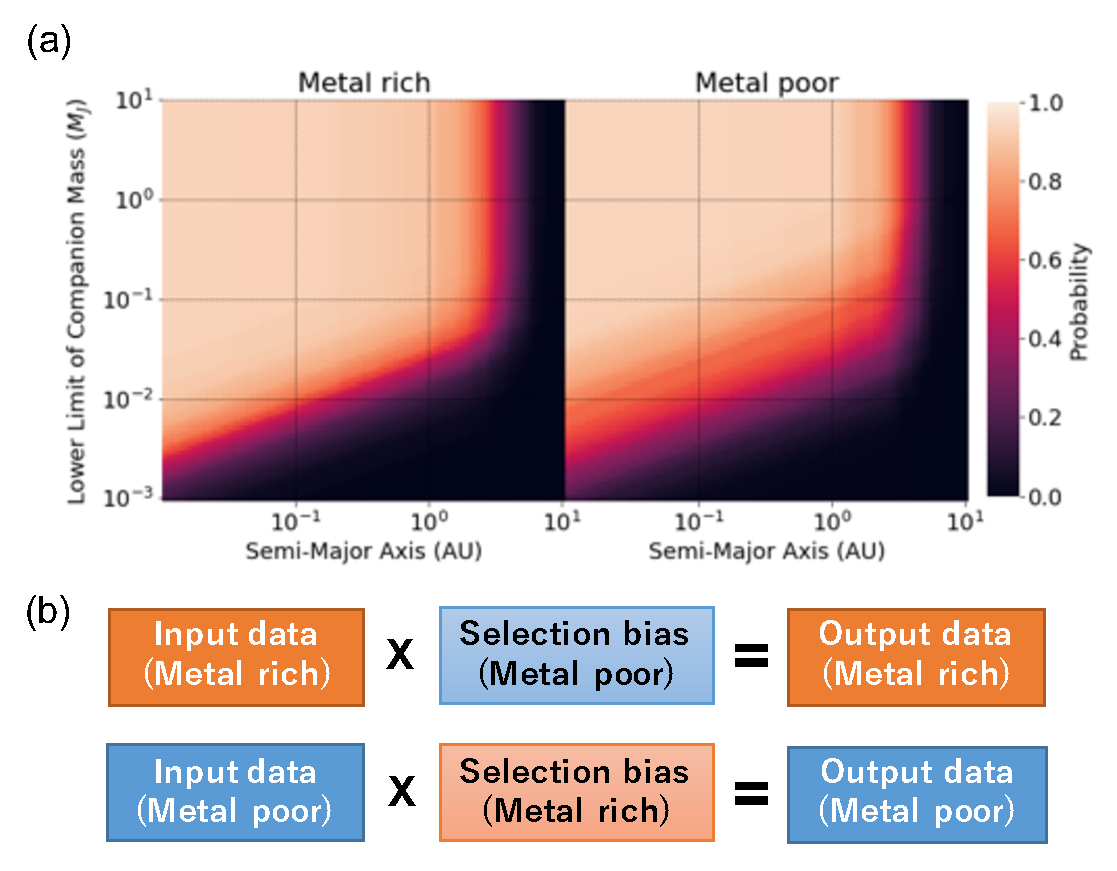
\includegraphics[width=9cm]{../../../Figure/selection_bias.pdf}
\caption{(a) The detectable regions for metal rich systems (left) and metal poor systems (right). The boundary of metallicity is fixed as 0.0 [Fe/H]. When a planetary system is observed, the only yellow regions can be detected. (b) The method of making dataset. Each data is filtered with the other's selection bias for flatting the difference of detection range. \label{fig:bias}}
\end{center}
\end{figure}


\section{Results} \label{sec:results}

In this section, we quantitively show how the effect of selection biases in different metal regions is, and classify the planetary distributions with Gaussian Mixture Model (GMM). We also discuss the differences of planetary-mass distributions and eccentricity distributions between the classified clusters.


\subsection{Planetary-mass distribution} \label{subsec:mass}

First, we determine the boundary of metallicity, which makes the two divided planetary-mass distributions most different, to verify the possibility of the effects due to the selection biases, and compare the two regions. Changing the metallicity boundary from -0.7 to 0.4 [Fe/H], we make the two regions' dataset, and evaluate the planetary-mass distributions with Anderson-Darling (AD) test (参考文献). Note that we extract randomly the values of planetary parameters with considering their errors, and filter randomly each sample with selection effects to remove the calculation bias. Then, the simulations are iterated until the boundary of metallicity is settled. As the result, we found that the best border of metallicity is -0.09 [Fe/H]. Dividing data with this result, we compare the planetary-mass distributions of both regions. The left of Figure \ref{fig:a_Mp}, (a) shows the relation between semi-major axes and planetary mass, and the right one is the cumulative of planetary mass. AD test for the metal rich and poor regions showed that the p-value was $5.6\times10^{-5}$, which can low enough to dismiss the two samples. Thus, we proposed that there are not any effects of selection bias for planetary-mass distribution, and exists a difference between the each metallicity region.

Second, we divide the planet samples into two regions with the optimized boundary of metallicity, and classify each planetary distribution with a classifier. In this time, we use GMM, which can classify the samples as the number of clusters with being assumed that each sample extend as a gaussian distribution \citep[e.g.,][]{2012MNRAS.424.2832L}. Converting the number of clusters, we evaluate each model with Bayesian Information Criterion (BIC), and find the best number of clusters for these samples. Then, both the samples in a metal rich and poor regions were optimized as the numbers of clusters were three, when the scores of BIC were 2644 and 1197, respectively.  Figure \ref{fig:a_Mp}, (b) shows the result of classification of planetary distribution with the best number of clusters. The black dash lines are the borders of planetary mass dividing the samples into three regions. These boundaries were drawn at 2.8 and 11.5 $M_J$ in a metal rich region, and 3.5 and 20.0 $M_J$ in a metal poor region, respectively.

\begin{figure}[t]
\begin{center}
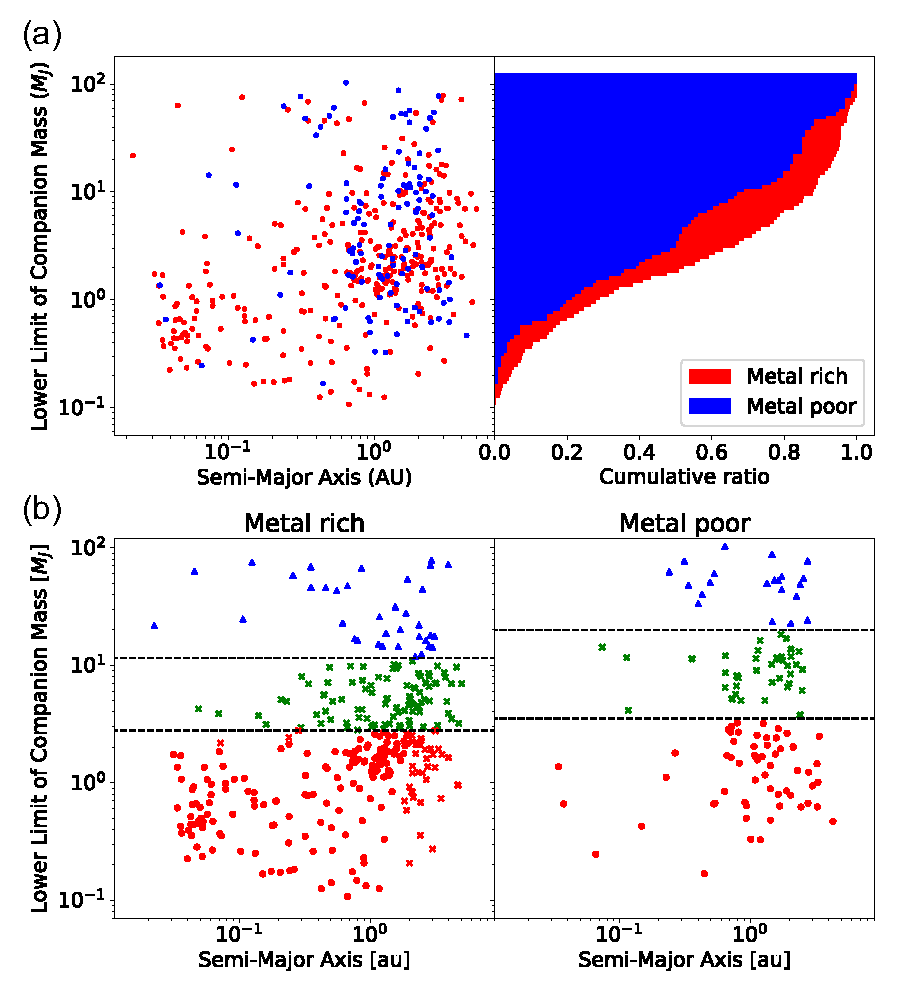
\includegraphics[width=9cm]{../../../Figure/a_Mp.pdf}
\caption{(a) The left is planetary distribution divided by the optimized boundary of metallicity. The red and blue points are the metal rich samples and metal poor ones, respectively. The right is the cumulative maps of the planetary masses in each region. Although the number of samples in a metal rich is a lot in a small mass field, the planets in a metal poor region are uniformly extending. (b) The result for classification of planetary distributions in each metal range with GMM. The marks in this figure are corresponding to each cluster label. The red, green, and blue points are used as the low-, middle-, and high-mass fields of planets. The black dash lines show the boundaries of planetary mass. \label{fig:a_Mp}}
\end{center}
\end{figure}


\subsection{Eccentricity distribution} \label{subsec:eccentricity}

The tops of Figure \ref{fig:e_Mp} are scatter maps of orbital eccentricities and planetary masses in each metal region after classification of planetary distribution with the mass boundaries obtained from GMM. The bottoms are the cumulative maps of the eccentricities in each region and cluster. In a metal poor range, the distribution of high-mass field is more uniform than any other field. This result is consistent with previous studies (参考文献). In contrast, the middle- and high-mass fields are extending as uniform. When the samples of low-mass field were compared with those of middle- or high-mass fields, the p-values were $1.6\times10^{-5}$ and $4.4\times10^{-4}$, respectively. (何かこの結果から推測できるものを書く?)

\begin{figure}[H]
\begin{center}
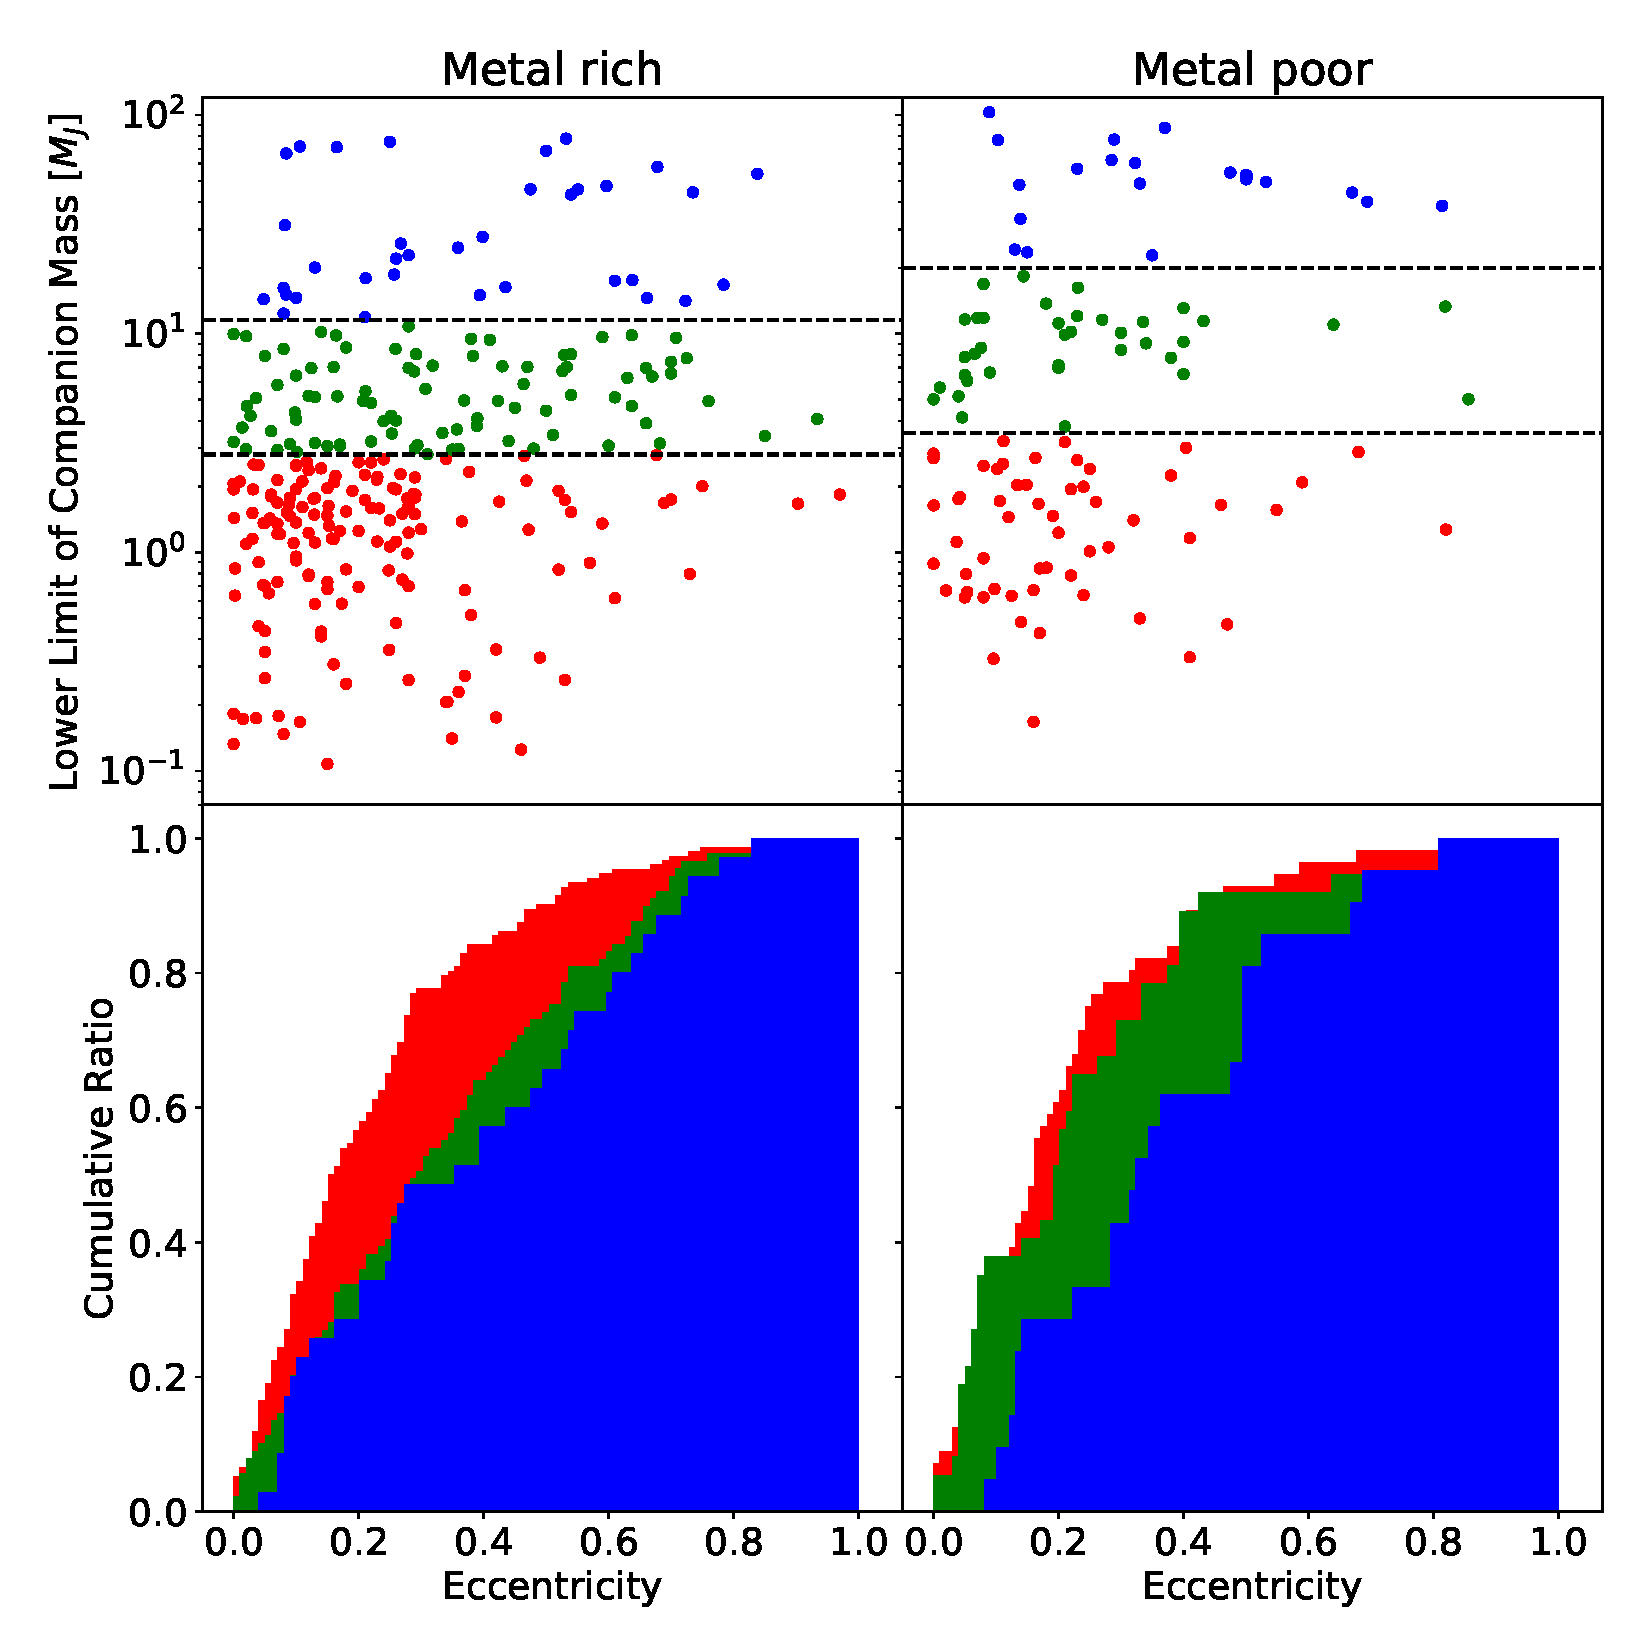
\includegraphics[width=9cm]{../../../Figure/e_Mp_merge.pdf}
\caption{Scatter maps of planetary eccentricities and masses (top), and cumulative maps of eccentricities (bottom). These colors are the same as those of Figure \ref{fig:a_Mp}, (b), and corresponding to the top and bottom figures. \label{fig:e_Mp}}
\end{center}
\end{figure}


\acknowledgments


\vspace{5mm}


\begin{thebibliography}{}

\bibitem[Boss(1997)]{1997Sci...276.1836B} Boss, A.~P.\ 1997, Science, 276, 1836
\bibitem[Boss(2002)]{2002ApJ...567L.149B} Boss, A.~P.\ 2002, \apjl, 567, L149
\bibitem[Buchhave et al.(2012)]{2012Natur.486..375B} Buchhave, L.~A., Latham, D.~W., Johansen, A., et al.\ 2012, \nat, 486, 375
\bibitem[Cai et al.(2006)]{2006ApJ...636L.149C} Cai, K., Durisen, R.~H., Michael, S., et al.\ 2006, \apjl, 636, L149
\bibitem[Calvi et al.(2011)]{2011MNRAS.416..727C} Calvi, R., Poggianti, B.~M., \& Vulcani, B.\ 2011, \mnras, 416, 727
\bibitem[Casagrande et al.(2011)]{2011A&A...530A.138C} Casagrande, L., Sch{\"o}nrich, R., Asplund, M., et al.\ 2011, \aap, 530, A138
\bibitem[Dodson-Robinson et al.(2009)]{2009ApJ...707...79D} Dodson-Robinson, S.~E., Veras, D., Ford, E.~B., \& Beichman, C.~A.\ 2009, \apj, 707, 79
\bibitem[Durisen et al.(2007)]{2007Arizona} Durisen, R. H., Reipurth, V. Jewitt, Keil, K., et al.\ 2007, Univ. of Arizona Press, Tucson 951, 607-622
\bibitem[Fischer \& Valenti(2005)]{2005ApJ...622.1102F} Fischer, D.~A., \& Valenti, J.\ 2005, \apj, 622, 1102
\bibitem[Hayashi\&Nakagawa(1985)]{1985Arizona} Hayahi, C., Nakazawa, K., \& Nakagawa, Y.\ 1985, Formation of the solar system. Protostars and Planets II. Tucson AZ, University of Arizona Press 1100-1153
\bibitem[Ida \& Lin(2004)]{2004ApJ...604..388I} Ida, S., \& Lin, D.~N.~C.\ 2004, \apj, 604, 388
\bibitem[Ida \& Lin(2004)]{2004ApJ...616..567I} Ida, S., \& Lin, D.~N.~C.\ 2004, \apj, 616, 567
\bibitem[Kuiper(1951)]{1951PNAS...37....1K} Kuiper, G.~P.\ 1951, Proceedings of the National Academy of Science, 37, 1
\bibitem[Lambrechts \& Johansen(2012)]{2012A&A...544A..32L} Lambrechts, M., \& Johansen, A.\ 2012, \aap, 544, A32
\bibitem[Lee et al.(2012)]{2012MNRAS.424.2832L} Lee, K.~J., Guillemot, L., Yue, Y.~L., Kramer, M., \& Champion, D.~J.\ 2012, \mnras, 424, 2832
\bibitem[Mayor \& Queloz(1995)]{1995Natur.378..355M} Mayor, M., \& Queloz, D.\ 1995, \nat, 378, 355
\bibitem[Mayer et al.(2002)]{2002Sci...298.1756M} Mayer, L., Quinn, T., Wadsley, J., \& Stadel, J.\ 2002, Science, 298, 1756
\bibitem[Mayer et al.(2007)]{2007ApJ...661L..77M} Mayer, L., Lufkin, G., Quinn, T., \& Wadsley, J.\ 2007, \apjl, 661, L77
\bibitem[Mayor et al.(2011)]{2011arXiv1109.2497M} Mayor, M., Marmier, M., Lovis, C., et al.\ 2011, arXiv:1109.2497
\bibitem[Mizuno(1980)]{1980PThPh..64..544M} Mizuno, H.\ 1980, Progress of Theoretical Physics, 64, 544
\bibitem[Mordasini et al.(2012)]{2012A&A...541A..97M} Mordasini, C., Alibert, Y., Benz, W., Klahr, H., \& Henning, T.\ 2012, \aap, 541, A97
\bibitem[Ormel \& Klahr(2010)]{2010A&A...520A..43O} Ormel, C.~W., \& Klahr, H.~H.\ 2010, \aap, 520, A43
\bibitem[Perri \& Cameron(1974)]{1974Icar...22..416P} Perri, F., \& Cameron, A.~G.~W.\ 1974, \icarus, 22, 416
\bibitem[Pollack et al.(1996)]{1996Icar..124...62P} Pollack, J.~B., Hubickyj, O., Bodenheimer, P., et al.\ 1996, \icarus, 124, 62
\bibitem[Santos et al.(2003)]{2003A&A...398..363S} Santos, N.~C., Israelian, G., Mayor, M., Rebolo, R., \& Udry, S.\ 2003, \aap, 398, 363
\bibitem[Torres et al.(2008)]{2008ApJ...677.1324T} Torres, G., Winn, J.~N., \& Holman, M.~J.\ 2008, \apj, 677, 1324
\bibitem[Wang \& Fischer(2015)]{2015AJ....149...14W} Wang, J., \& Fischer, D.~A.\ 2015, \aj, 149, 14
\bibitem[Weiss et al.(2013)]{2013ApJ...768...14W} Weiss, L.~M., Marcy, G.~W., Rowe, J.~F., et al.\ 2013, \apj, 768, 14
\bibitem[Young(2003)]{2003NewAR..47....1Y} Young, R.~E.\ 2003, \nar, 47, 1

\end{thebibliography}

%\appendix

\end{CJK*}
\end{document}
